\documentclass[11pt,a4paper]{article}
\usepackage[margin=2.4cm]{geometry}
\usepackage{graphicx}
\usepackage{amsmath}
\usepackage{amssymb}
\usepackage{xcolor}
\usepackage[colorlinks=true,linkcolor=blue!50!black,urlcolor=blue!50!black,citecolor=blue!50!black]{hyperref}
\graphicspath{{figs/}}

\newcommand{\He}[1]{$^{#1}$He}
\newcommand{\sM}{\sigma_{\mathrm{M1}}}
\newcommand{\sE}{\sigma_{\mathrm{E0}}}

\title{\vspace{-1.2cm}
  {\Large\bfseries The E0 pair channel in \He{3}$(n,\cdot)$\He{4}}\\[2mm]
  {\large Broken into two parts --- \emph{which} excited state we form, and
   \emph{how} it decays --- to find a second, $\gamma$-dark source of
   $e^+e^-$ pairs}}
\author{Dylan Neff}
\date{15 June 2026 \\[2mm]
  {\small\itshape Internal note --- informal. Drafted by Claude (Anthropic AI
  assistant) under D.~Neff's direction; \\ physics, numbers and text
  reviewed by D.~Neff.}}

\begin{document}
\maketitle
\vspace{-0.8cm}

%=============================================================================
\section*{Part 0 --- Summary}

\begin{center}
\fcolorbox{blue!40!black}{blue!4}{%
\begin{minipage}{0.95\textwidth}
\vspace{3pt}
\textbf{The problem splits cleanly into two parts, linked by the spin-parity
$J^\pi$ of the intermediate \He{4}$^*$ state:}
\begin{itemize}\setlength\itemsep{1pt}
  \item \textbf{Part 1 --- Formation:} which \He{4}$^*$ state does the captured
    neutron make, vs energy? Set by angular momentum (s-wave $\to0^+,1^+$;
    p-wave $\to0^-,2^-,1^-$). \textbf{This sets the energy \emph{shape}.}
  \item \textbf{Part 2 --- Decay:} given that state, how does it reach the $0^+$
    ground state and does it make a pair? Set by selection rules.
    \textbf{This sets the \emph{height} (pair fraction).}
\end{itemize}
\textbf{Key results:}
(i) Only \emph{three} states make ground-state pairs: $0^+$ (E0, \textbf{100\,\%
pairs}, $\gamma$-dark), $1^+$ (M1) and $1^-$ (E1, both 0.35\,\% pairs). $0^-$
and $2^-$ are spectators.
(ii) A $0^+\!\to0^+$ transition can go \emph{only} by E0 --- not M1 (the $0\to0$
rule forbids both the photon and M1). The M1 is a \emph{different} capture
channel.
(iii) \textbf{There is no low-lying $1^+$ level} --- the lowest is $\sim$28 MeV,
so the M1 capture is \emph{direct} (non-resonant) through the continuum; the
$0^+$ is the only state with a (sub-threshold) resonance helping it.
(iv) The \He{4} levels are so broad ($\Gamma\gtrsim|E_r|$) that capture is
\textbf{mostly direct/continuum}, not sharp resonant capture --- except for a
real, broad sub-threshold boost of the E0 at low $E_n$ ($\sim$10$\times$).
(v) The E0 and M1/E1 pairs sit at \emph{opposite} ends of the energy range
(E0 low, M1/E1 MeV); the absolute E0 size is the one unknown,
$f=\sE/\sM\sim10^{-3}$--$10^{-2}$.
\vspace{3pt}
\end{minipage}}
\end{center}

%=============================================================================
\section*{Part 1 --- Formation: which \He{4}$^*$ state do we make?}

A slow neutron and \He{3} fuse into \He{4}$^*$ at $\approx$20.6\,MeV. Which
excited state forms depends on energy; \emph{whether it makes a pair} is decided
later (Part 2).

\subsection*{The states that exist --- and the $1^+$ surprise}

\begin{center}
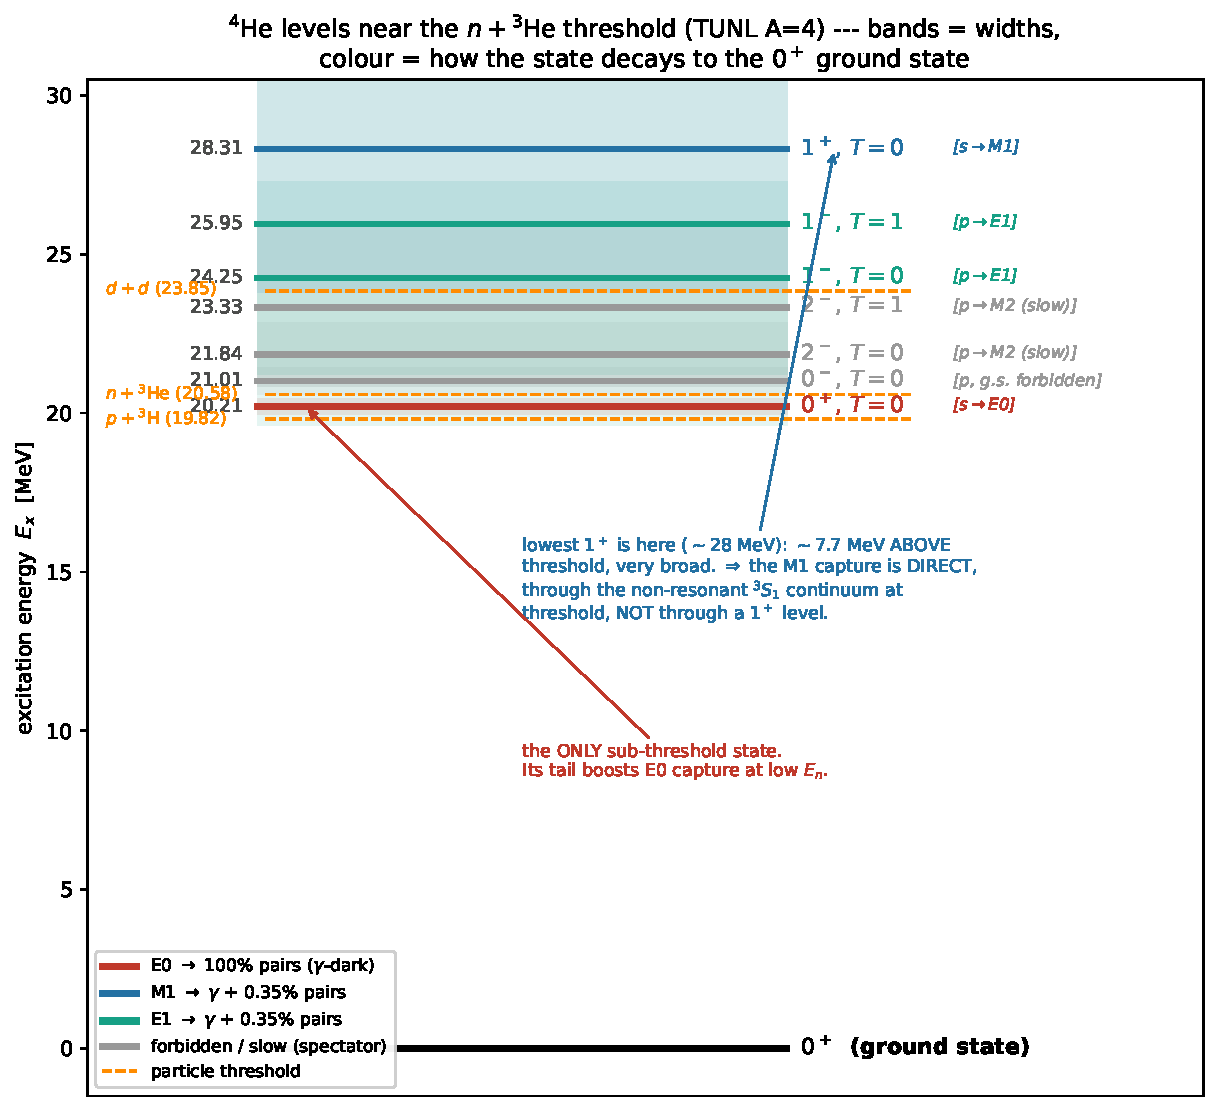
\includegraphics[width=0.86\textwidth]{fig_e0_levels.pdf}
\end{center}

\noindent The \He{4} levels near the $n+{}$\He{3} threshold (20.58\,MeV), from
the TUNL $A=4$ evaluation \cite{tunl}. Two things to read off:
\begin{itemize}\setlength\itemsep{1pt}
  \item The levels are \textbf{broad and overlapping} (widths 0.5--13\,MeV) ---
    \He{4} has no sharp levels above threshold.
  \item \textbf{There is no low-lying $1^+$ state.} The lowest $1^+$ is at
    $\sim$28.3\,MeV --- about 7.7\,MeV \emph{above} threshold and very broad.
    (This is the answer to ``where is the $1^+$?'' --- it simply isn't down here.)
\end{itemize}

\subsection*{Which state, and when: angular momentum}

Parity fixes the entrance orbital angular momentum, $\pi=(-1)^\ell$:
\begin{center}
\begin{tabular}{lll}
\hline
reached by & $\to$ states & energy behaviour \\
\hline
\textbf{s-wave} ($\ell=0$) & $0^+,\,1^+$ & no barrier --- rise as $1/v$, \textbf{dominate at low $E_n$} \\
\textbf{p-wave} ($\ell=1$) & $0^-,\,2^-,\,1^-$ & barrier-suppressed --- \textbf{switch on at sub-MeV/MeV} \\
\hline
\end{tabular}
\end{center}

\begin{center}
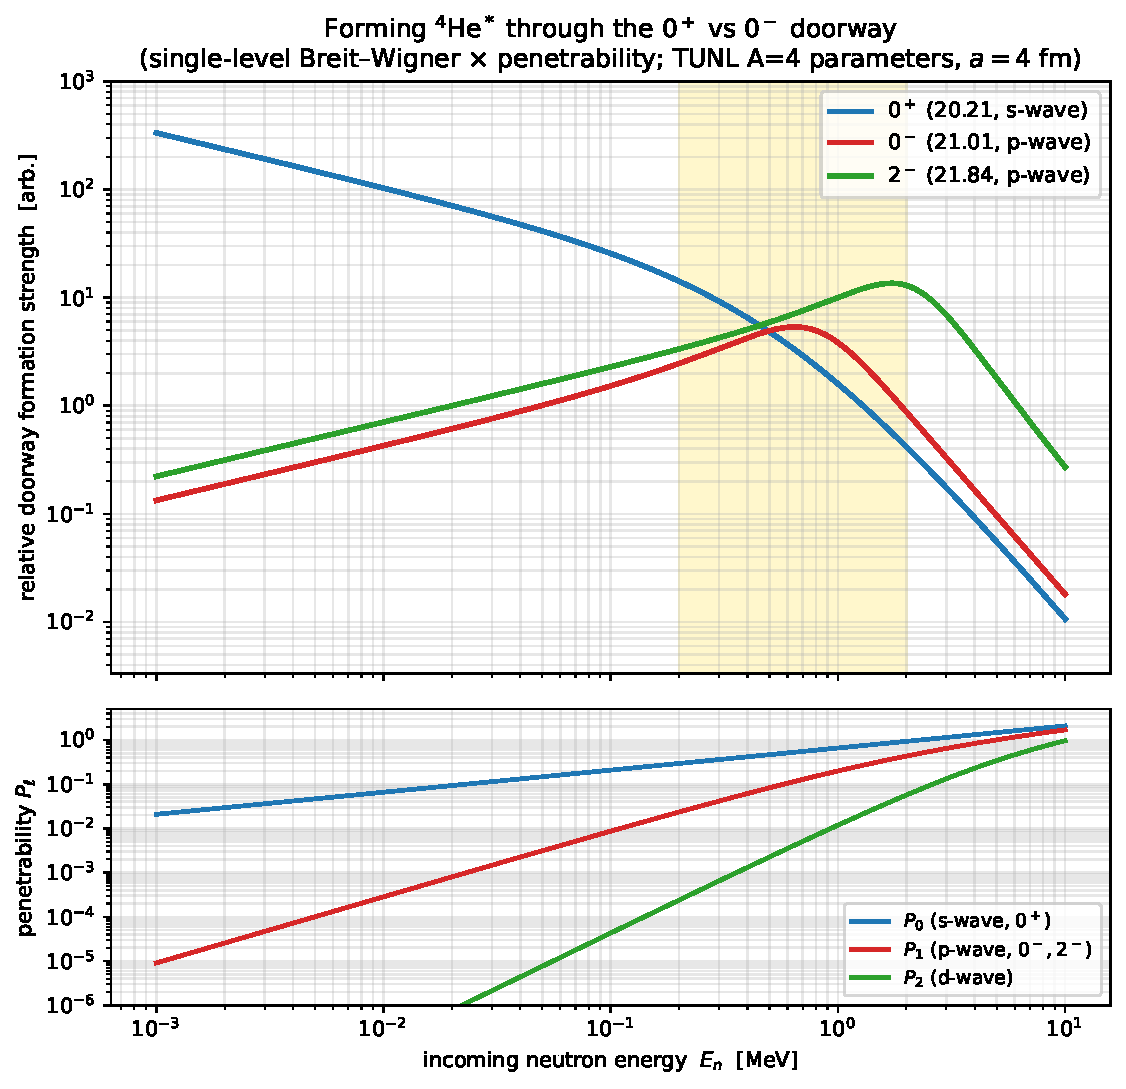
\includegraphics[width=0.78\textwidth]{fig_e0_doorway.pdf}
\end{center}

\noindent Both $0^+$ and $1^+$ (s-wave) dominate at low $E_n$; $0^-$ and $2^-$
(p-wave) peak at $E_n\approx0.6$ and $\approx1.7$\,MeV --- \emph{not} forbidden
at low energy, just barrier-suppressed. \textbf{As the neutron energy drops, we
form relatively more $0^+$ and $1^+$.}

\subsection*{Continuum (direct) vs resonance}

Is this capture \emph{resonant} (through a sharp level) or \emph{direct}
(into the continuum, the photon emitted during scattering)? A level acts as a
sharp resonance only if its width is smaller than its distance from the capture
window, $\Gamma<|E_r|$. For \He{4} that is never the case
(Fig.~\ref{fig:dr}): every level has $\Gamma/|E_r|\approx1.2$--1.9, so
\textbf{the capture is mostly direct/continuum capture}, modulated by broad
structures, not sharp resonant capture. Two consequences matter for us:

\begin{figure}[h]
\centering
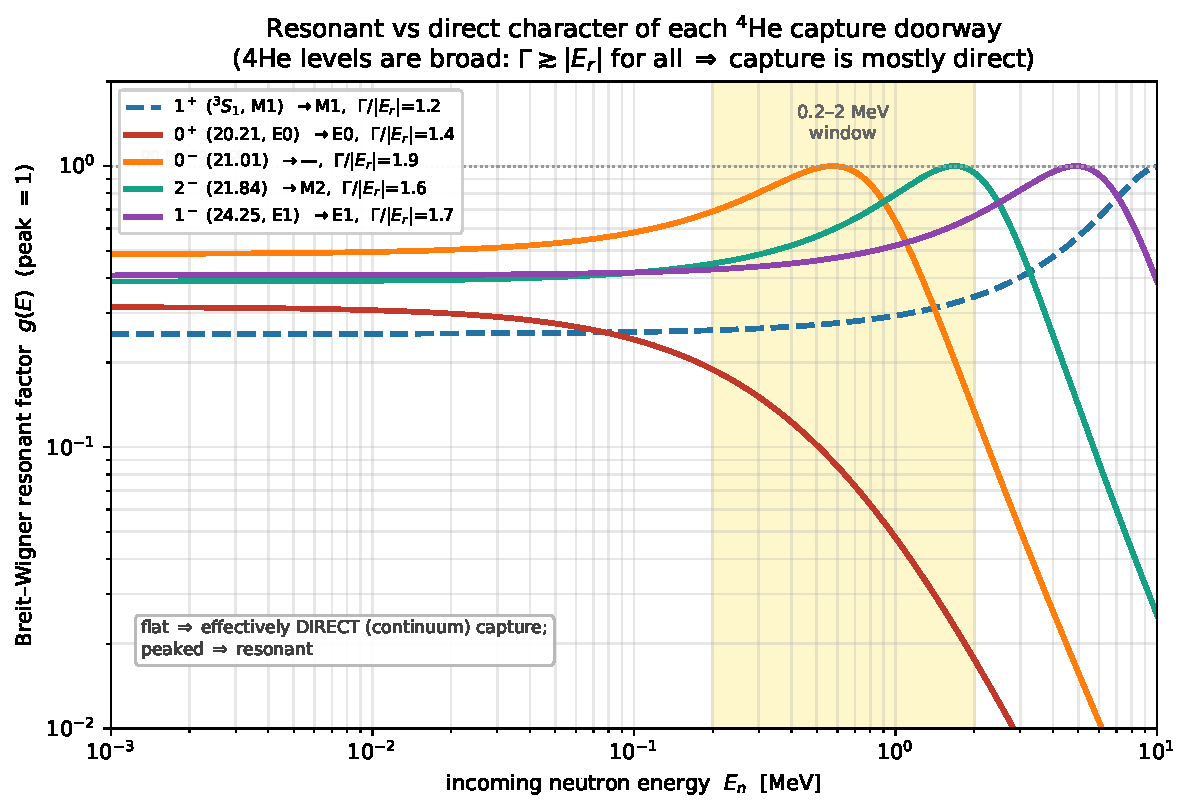
\includegraphics[width=0.80\textwidth]{fig_e0_directres.pdf}
\caption{How ``resonant'' each doorway is across the capture window: the
  Breit--Wigner factor $g(E)$ (peak $=1$). \textbf{Flat $\Rightarrow$ effectively
  direct} (continuum) capture; \textbf{peaked $\Rightarrow$ resonant}.}
\label{fig:dr}
\end{figure}

\begin{itemize}\setlength\itemsep{1pt}
  \item \textbf{$1^+$ (M1): pure direct.} Its nearest level is 7.7\,MeV away and
    9\,MeV wide, so $g(E)$ is flat ($g_{\rm thr}/g_{1\,\rm MeV}\approx0.8$): the
    famous 54\,$\mu$b M1 capture is \emph{direct continuum capture}, with no
    resonant enhancement. (This is why \He{3}$(n,\gamma)$ follows a clean $1/v$
    with no thermal resonance.)
  \item \textbf{$0^+$ (E0): direct $+$ a sub-threshold boost.} The 20.21\,MeV
    $0^+$ sits 0.37\,MeV \emph{below} threshold; its tail enhances the E0
    capture by $\sim$10$\times$ at threshold relative to 1\,MeV --- a real, but
    \emph{broad}, resonant boost concentrated at the lowest $E_n$.
  \item $0^-,2^-,1^-$ (p-wave) peak in the sub-MeV/MeV region and only matter
    there.
\end{itemize}

%=============================================================================
\section*{Part 2 --- Decay: what does each state do?}

Whatever state forms, \He{4}$^*$ almost always just \textbf{breaks back up}
($p+{}^3$H, the (n,p)t reaction, or $n+{}$\He{3}) and makes no pair. The rare
($10^{-8}$--$10^{-4}$) \textbf{electromagnetic drop to the $0^+$ ground state} is
the only pair source, and \emph{what kind} of drop is fixed by the state's
$J^\pi$. Taking each state on its own:

\begin{center}
\renewcommand{\arraystretch}{1.25}
\begin{tabular}{llcl}
\hline
State & $\to0^+$ g.s. & pairs? & role for our signal \\
\hline
\textbf{$0^+$} (20.21) & \textbf{E0} ($\gamma$ forbidden) & \textbf{100\,\%} & \textbf{E0 pair source} --- low $E_n$ \\
\textbf{$1^+$} ($^3S_1$) & M1 & 0.35\,\% & \textbf{M1 pair source} --- the ordinary 54\,$\mu$b \\
\textbf{$1^-$} (24--26) & E1 & 0.35\,\% & \textbf{E1 pair source} --- rises toward MeV \\
$0^-$ (21.01) & forbidden & --- & spectator (breaks up) \\
$2^-$ (21.84) & M2 (too slow) & $\sim$0 & spectator \\
\hline
\end{tabular}
\end{center}

\noindent Row by row:
\begin{itemize}\setlength\itemsep{1pt}
  \item \textbf{$0^+\to0^+$: E0.} A photon is forbidden ($0\to0$), so the
    \emph{only} outlet is an $e^+e^-$ pair --- \textbf{100\,\% of these
    transitions are pairs.} This is the $\gamma$-dark channel, invisible to
    ENDF/Geant4 (and absent from our generator).
  \item \textbf{$1^+\to0^+$: M1.} Emits a 20.6\,MeV $\gamma$; $\sim$0.35\,\% of
    those convert to a pair (the internal-pair coefficient
    $\alpha_{\rm IPC}\approx3.5\times10^{-3}$ at this energy, anchored to the
    \emph{measured} $^{12}$C 15.1\,MeV M1 value $(3.3\pm0.5)\times10^{-3}$
    \cite{ipc12c}; BrIcc's tables stop at 6\,MeV \cite{bricc}).
  \item \textbf{$1^-\to0^+$: E1.} Same as M1 (a $\gamma$ with a 0.35\,\% pair
    tail), but p-wave, so it grows toward MeV --- this is what makes the
    radiative cross section rise (the giant dipole turning on).
  \item \textbf{$0^-\to0^+$: nothing.} $0\to0$ forbids every photon multipole,
    and a parity flip forbids E0 too --- so the $0^-$ has no electromagnetic
    route to the ground state and simply decays back to particles. A pure
    spectator (even though it peaks near 0.6\,MeV).
  \item \textbf{$2^-\to0^+$: M2,} far too slow at 20\,MeV; the state breaks up
    first. Spectator.
\end{itemize}

%=============================================================================
\section*{Putting the two parts together}

\textbf{Part 1 sets the shape, Part 2 sets the height}, and the total pair yield
is the sum over the three source states,
$N_{\rm pairs}(E_n)=\sum_{J^\pi}[\text{formation}(J^\pi,E_n)]\times[\text{pair
fraction}(J^\pi)]$. The two pair families end up at opposite ends of the energy
range:

\begin{center}
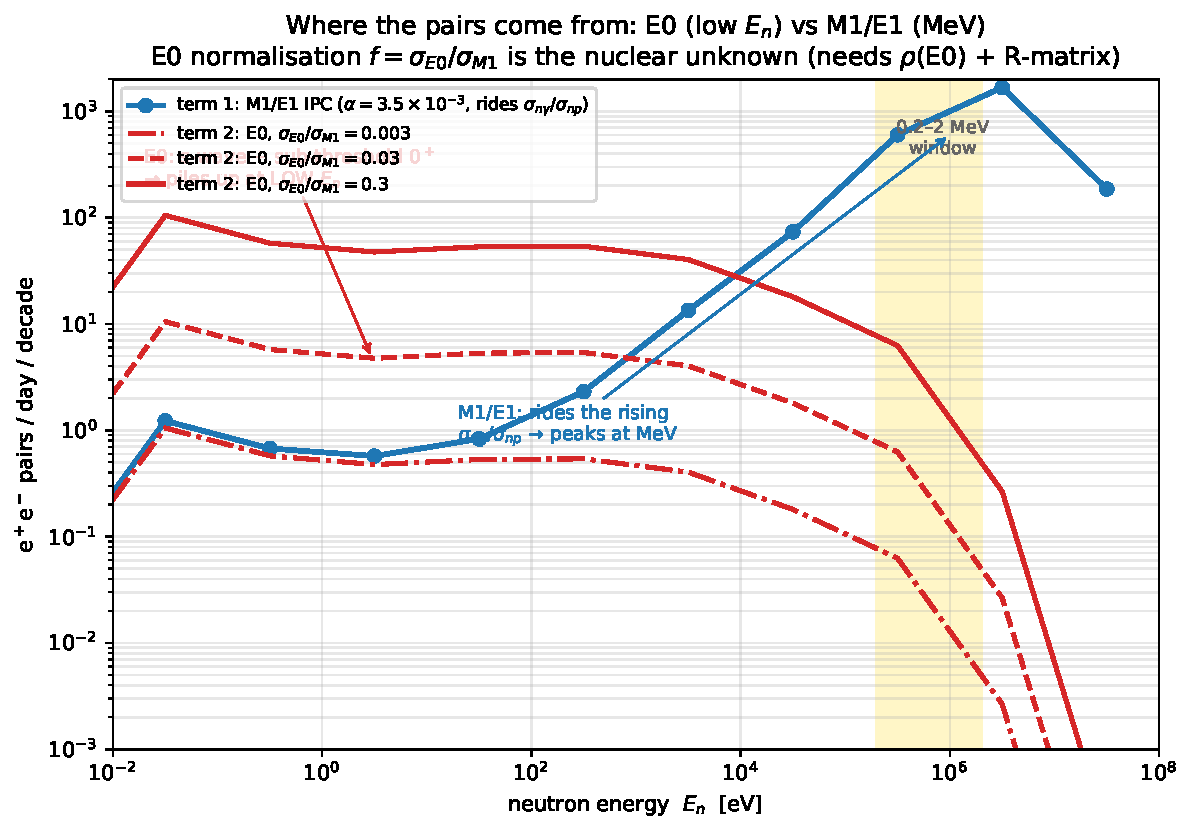
\includegraphics[width=0.84\textwidth]{fig_e0_yield.pdf}
\end{center}

\begin{itemize}\setlength\itemsep{1pt}
  \item \textbf{M1/E1 (blue):} 0.35\,\% pair fraction, but rides the rising
    radiative cross section $\Rightarrow$ \textbf{peaks at MeV}. This is the
    piece we can already compute ($\approx$2200 pairs/day, $0.1$--10\,MeV).
  \item \textbf{E0 (red):} 100\,\% pair fraction \emph{and} the low-energy
    s-wave + sub-threshold boost $\Rightarrow$ \textbf{piles up at thermal /
    sub-keV.}
\end{itemize}

\noindent So \textbf{the sub-keV region we had written off (for M1 it is dead)
might be exactly where the E0 pairs live} --- a genuinely different place to
look.

\subsection*{The one unknown: the height of the E0 curve}

Everything above is settled except \emph{how strong} the E0 channel is, i.e.\
$f=\sE/\sM$ --- physically, how often the $0^+$ doorway makes its E0 transition
to the ground state rather than breaking up. A literature dig found: the \He{4}
$0^+_2$ E0 strength \emph{is} measured (the MAMI monopole form factor
\cite{kegel}, the ``$\alpha$-particle monopole puzzle'' \cite{puzzle}) and is a
real, collective transition --- but that is the \emph{decay-side} matrix element;
turning it into a capture rate needs reaction theory. The ATOMKI \He{4} pair
work \cite{atomki} models its pairs as E1/M1 capture, not a clean E0 line, and
no calculation of \He{3}$(n,e^+e^-)$\He{4} exists. A transparent
order-of-magnitude argument (statistical $^1S_0$ weight $\tfrac14$ as a floor;
E0 having no real-photon mode as a ceiling) brackets
\[
\boxed{\,f=\sE/\sM\sim10^{-3}\text{--}10^{-2}\,}\quad\Longrightarrow\quad
\frac{\text{E0 pairs}}{\text{M1 pairs}}=\frac{f}{\alpha_{\rm IPC}}\sim0.3\text{--}3
\]
at low $E_n$ --- E0 plausibly \emph{same-order-or-larger} than the M1 pairs in
the sub-keV. The clean way to replace the bracket with a number is a \He{4}
multi-level R-matrix (Hale's evaluated system) for the $^1S_0$ capture,
normalised by the measured $(e,e')$ strength. \emph{Next step, worth doing
together.}

\subsection*{What this sets up}
With the shapes (Part 1) and pair fractions (Part 2) in hand, the remaining step
is to fold in the absolute normalisations and the detector acceptance to get the
final metric --- X17 / IPC pairs per pulse (per day) vs neutron energy --- now
\emph{including} the E0 channel. That is the next note.

%=============================================================================
\section*{Reproducing the figures}
{\raggedright
Scripts (in \texttt{scripts/}): levels --- \texttt{make\_he4\_levels\_fig.py};
doorways --- \texttt{calc\_doorway\_formation.py}; direct-vs-resonant ---
\texttt{calc\_direct\_vs\_resonant.py}; pair yield ---
\texttt{make\_e0\_pair\_yield\_fig.py}.
Companion markdown (in \texttt{docs/e0\_branch/}): the spine is
\texttt{formation\_and\_decay.md}; see also \texttt{capture\_breakdown.md},
\texttt{doorway\_states\_note.md}, \texttt{ipc\_estimation\_method.md}, and
\texttt{ipc\_roadmap.md}.
\par}

\begin{thebibliography}{9}
\small\sloppy
\bibitem{tunl} D.~R.~Tilley, H.~R.~Weller, G.~M.~Hale, ``Energy levels of
  $A=4$'', Nucl.\ Phys.\ A \textbf{541} (1992) 1 (TUNL); G.~M.~Hale's \He{4}
  R-matrix.
\bibitem{kegel} S.~Kegel \emph{et al.}, ``Measurement of the $\alpha$-Particle
  Monopole Transition Form Factor'', Phys.\ Rev.\ Lett.\ \textbf{130} (2023)
  152502 (MAMI A1).
\bibitem{puzzle} ``Derivation of transition density from the observed
  \He{4}$(e,e')$\He{4}$(0^+_2)$ form factor \dots'', arXiv:2306.07268;
  arXiv:2406.00653.
\bibitem{atomki} A.~J.~Krasznahorkay \emph{et al.}, ``New anomaly observed in
  \He{4} \dots'', Phys.\ Rev.\ C \textbf{104} (2021) 044003; arXiv:2104.10075.
\bibitem{bricc} T.~Kib\'edi \emph{et al.}, BrIcc, Nucl.\ Instrum.\ Meth.\ A
  \textbf{589} (2008) 202; \url{https://github.com/IAEA-NSDDNetwork/BrIcc}
  (pair coefficients tabulated only to 6\,MeV).
\bibitem{ipc12c} Measured $^{12}$C 15.1\,MeV M1 IPC, $\alpha_\pi=(3.3\pm0.5)
  \times10^{-3}$ (PEPSI; arXiv:nucl-ex/9704007).
\bibitem{ss} M.~Schl\"uter, G.~Soff, W.~Greiner, Z.~Phys.\ A \textbf{286} (1978)
  149; At.\ Data Nucl.\ Data Tables \textbf{24} (1979) 509 (high-energy IPC).
\bibitem{werv} R.~Wervelman \emph{et al.}, \He{3}$(n,\gamma)$\He{4} M1/E1
  content, Nucl.\ Phys.\ A \textbf{526} (1991) 265.
\end{thebibliography}

\end{document}
